% !TEX encoding = UTF-8 Unicode
% !TEX spellcheck = en-US


% This is the root file of your thesis: thesis.tex
% A line starting with % is a comment. In some cases, I have included a command preceded by a %. You may activate the command by removing the %.

%%===================================
\documentclass[12pt]{report}
\usepackage[T1]{fontenc} 			
\usepackage{graphicx}
\usepackage{color}
\usepackage{transparent}
%\usepackage{stackengine}
\usepackage{booktabs}
\usepackage{amsmath,amssymb} 
\usepackage{textcomp}
\usepackage{hyperref}
\usepackage[capitalize]{cleveref}
\usepackage{subcaption}
\usepackage{siunitx}				
	\sisetup{exponent-product = \cdot}      
	\sisetup{output-decimal-marker  =  {.}} 	
	\sisetup{separate-uncertainty = true}   	

%%===================================
%Write the various parts of your thesis as separate files and include them into the main file by the command \include{name of included file}. When you compile the LaTeX file, you may choose which subfiles to include by the command

%\includeonly{chapter01,chapter02}

%%===================================
\begin{document}
% !TEX encoding = UTF-8 Unicode
%!TEX root = thesis.tex
% !TEX spellcheck = en-US

%This is the Titlepage
%%=========================================
\thispagestyle{empty}
\mbox{}\\[6pc]
\begin{center}
\Huge{This is the Title of my Thesis}\\[2pc]

\Large{Your Name}\\[1pc]
\large{August 2014}\\[2pc]

PROJECT / MASTER THESIS\\
Department of Production and Quality Engineering\\
Norwegian University of Science and Technology
\end{center}
\vfill

\noindent Supervisor: Professor Ask Burlefot


 % This is the titlepage
\setcounter{page}{0}
\pagenumbering{roman}
% !TEX encoding = UTF-8 Unicode
%!TEX root = thesis.tex
% !TEX spellcheck = en-US
%%=========================================
\addcontentsline{toc}{section}{Preface}
\section*{Preface}
Here, you give a brief introduction to your work. What it is (e.g., a Master's thesis in RAMS at NTNU as part of the study program xxx and\ldots), when it was carried out (e.g., during the autumn semester of 2021). If the project has been carried out for a company, you should mention this and also describe the cooperation with the company. You may also describe how the idea to the project was brought up.

You should also specify the assumed background of the readers of this report (who are you writing for).\\[2cm]

\begin{center}
Trondheim, 2012-12-16\\[1pc]
(Your signature)\\[1pc]
Ola Nordmann
\end{center}
% !TEX encoding = UTF-8 Unicode
%!TEX root = thesis.tex
% !TEX spellcheck = en-US
%%=========================================
\addcontentsline{toc}{section}{Acknowledgment}
\section*{Acknowledgment}
I would like to thank the following persons for their great help during \ldots

If the project has been carried out in cooperation with an external partner (e.g., a company), you should acknowledge the contribution and give thanks to the involved persons.

You should also acknowledge the contributions made by your supervisor(s).

\begin{flushright}
O.N.\\[1pc]
(Your initials)
\end{flushright}
% !TEX encoding = UTF-8 Unicode
%!TEX root = thesis.tex
% !TEX spellcheck = en-US
%%=========================================
\addcontentsline{toc}{section}{Summary and Conclusions}
\section*{Summary and Conclusions}
Here you give a summary of your your work and your results. This is like a management summary and should be written in a clear and easy language, without many difficult terms and without abbreviations. Everything you present here must be treated in more detail in the main report. You should not give any references to the report in the summary -- just explain what you have done and what you have found out. The Summary and Conclusions should be no more than two pages.

You may assume that you have got three minutes to present to the Rector of NTNU  what you have done and what you have found out as part of your thesis. (He is an intelligent person, but does not know much about your field of expertise.)
\tableofcontents
\setcounter{page}{0}
\pagenumbering{arabic}
% !TEX encoding = UTF-8 Unicode
%!TEX root = thesis.tex
% !TEX spellcheck = en-US
%%=========================================
\chapter{Introduction}

\chapter{Theory}

\section{Electron Microscopy}
In an electron microscope, a beam of electrons are transmitted onto a material. Compared to a microscope using visible light, an EM gives a much higher resolution due to the wavelength of electrons being much smaller than that of visible light. Because of this, an EM can be used to study the atomic structure of materials.

	\subsection{Electron-sample interaction}
When the electron beam hits the sample, several different signals are generated. This report will only discuss two of them: Characteristic X-rays (due to inelastically scattered electrons, and elastically scattered electrons. Characteristic X-rays are produced as the incoming electrons interact with inner-core electrons in the sample, and can be used to determine which elements the sample consists of. The theory behind characteristic X-rays, and why they are useful, will be expanded upon in section \ref{EDS}. Electrons being transmitted through the sample that are elastically scattered (that is, the energy of the incoming electrons is conserved) gives rise to a diffraction pattern, which can be used to determine the crystallographic properties of the sample. Electron diffraction will be properly introduced in section \ref{ED} \cite{williams-carter}.

	\subsection{Transmission Electron Microscopy (TEM)}
There are many different kinds of transmission electron microscopes (TEMs), of which only the scanning TEM (STEM), introduced in section \ref{STEM}, will be expanded upon here. Before discussing the STEM, however, the basics behind the TEM will now be presented. In a conventional TEM, a broad, parallel beam of electrons is transmitted through a sample. In order for a sufficient amount of electrons to be transmitted, the sample is required to be thin (a thickness of <$\SI{100}{\nano\meter}$ is common). A TEM typically operates with electron energies of $\SI{200}{\kilo\electronvolt}$ or $\SI{300}{\kilo\electronvolt}$, giving the electrons a velocity $v > c/2$ which requires relativistic effects to be taken into account. Another factor that should be considered is the possibility of the electron beam damaging the material. This can happen as the chemical bonds in the material are broken (radiolysis), atoms are displaced or ejected from the crystal lattice (knock-on damage or sputtering, respectively) or as the material is changed due to heating. \cite{williams-carter}

%	\subsection{Scanning Electron Microscopy (SEM)}

	\subsection{Scanning Transmission Electron Microscopy (STEM)}
A scanning transmission electron microscope (STEM) uses an electron beam focused onto a small spot on the sample. The sample is then scanned in a raster pattern and the signal is recorded for each point. This technique can be used to investigate very small areas of the sample and accurately study transitions in atomic structure and/or composition.

\section{X-ray spectroscopy}\label{EDS}
The characteristic X-rays resulting from inelastic scattering of the electrons being transmitted through the sample can be used for both qualitative and quantitative analysis. Qualitative analysis can determine which elements are in the sample, while quantitative analysis can indicate the composition of the different elements. When X-ray spectroscopy is performed in a STEM, the electron probe is scanned over the material and focused on each pixel for a certain amount of time. During this time period, the X-rays being emitted from the sample are detected and the signal for the pixel is saved before the probe moves to the next pixel. 

	\subsection{Energy-Dispersive X-Ray Spectroscopy (EDS)} % Taken in STEM!!
		\subsubsection{X-ray emission}
As previously mentioned, characteristic X-rays are produced due to inelastic scattering of the incoming electrons on the sample. If an electron reaches the inner-shell electrons of an atom in the sample, and a sufficient amount of energy is transferred to the inner-shell electron, the electron will be ejected from the nucleus. That is, it reaches an energy above the Fermi level and is no longer bound to the nucleus [CHECK THIS]. The atom is now in an excited state, and will seek to return towards its ground state. This leads to an electron in an outer shell taking the place of the ejected electron in the inner shell, and in the process emitting an X-ray or an Auger electron (Auger electrons will not be discussed further). If an X-ray is emitted, its energy will be characteristic of the specific element, as different elements have different critical ionization energies. The critical ionization energy is the energy required for an inner-shell electron to be ejected from the nucleus.

There will not necessarily only be emitted one characteristic X-ray for each hole created in the inner shell of an atom. This is because the outer-shell electron filling the hole will create a new hole in its shell, which must be filled by an electron in a shell even further out, and maybe emitting another characteristic X-ray. This process continues until there is a hole in the outermost shell of the atom that can be filled by an electron in the conduction or valence band of the material. The energy of the characteristic X-rays will also depend on which transition it is emitted because of. In addition, due to quantum effects the electron shells might be split into several sub-shells, further increasing the number of different energies the emitted X-rays can have.

The probability for a specific transition to occur must also be taken into account. If a transition between two specific shells has a relatively high probability compared to other transitions in the element, more characteristic X-rays with the corresponding energy will be emitted over a certain time period. This will lead to higher peaks in the EDS spectrum, which will be discussed shortly.

		\subsubsection{X-ray detection}
When doing EDS in a TEM, an X-ray detector is positioned above the sample to detect the X-rays emitted from it. The detector then measures the energy of each incoming X-ray, with a given energy resolution. If the measurement is done using STEM, the electron probe is scanned over the sample and kept at each pixel for a certain amount of time during which emitted X-rays are detected. When the scanning is complete, this results in a three dimensional EDS spectrum.

		\subsubsection{EDS spectrum}\label{sec:eds-spec}
In an EDS spectrum, the intensity of the X-rays is plotted against the energy of the X-rays. The intensity at a certain energy refers to the number of counts, that is, how many X-rays with that energy that were detected by the detector. An example of an EDS spectrum is shown in Figure \ref{fig:eds-example-spectrum}. By consulting a table of known X-ray energies for the emission lines from different elements, for example \cite{x-ray-booklet}, one can determine which elements are present in the sample. However, knowing which elements are present is not enough to determine the structure of the material. A next step can be to perform quantitative analysis on the same spectrum.

\begin{figure}
\centering
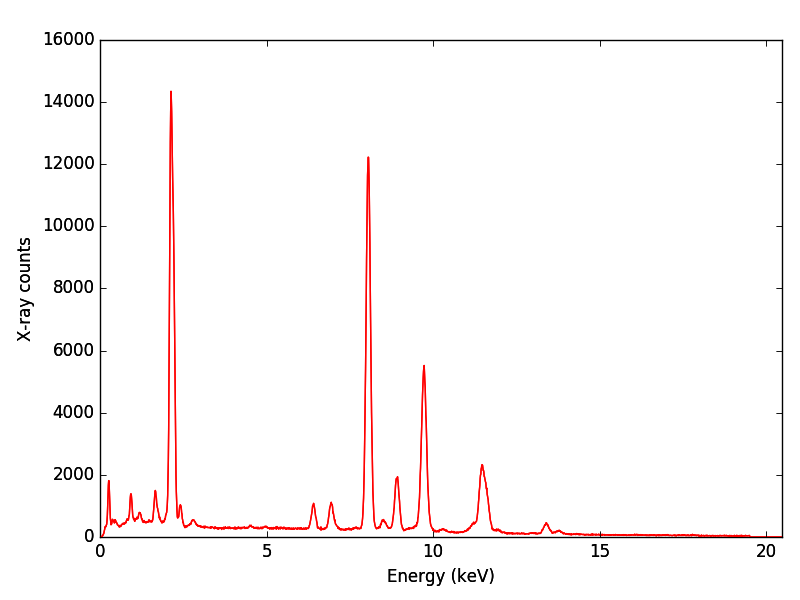
\includegraphics[width=0.7\linewidth]{fig/edx-example-spectrum}
\caption{Example of EDS spectrum}
\label{fig:eds-example-spectrum}
\end{figure}

	\subsection{Quantitative X-ray Analysis}
Quantitative analysis of an EDS spectrum gives information about the composition of the different elements in the material. A quantitative analysis might result in learning that an unknown material is a compound of a few different elements. In order to determine which compound this is, quantitative analysis is necessary.

There are primarily two methods for quantitative X-ray analysis: The Cliff-Lorimer ratio technique and the $\zeta$-factor method. The basis for both is assuming that the concentration of an element in a material is proportional to the intensity of characteristic X-rays being emitted from it, $C \propto I$.

		\subsubsection{The Cliff-Lorimer ratio technique}
The Cliff-Lorimer ratio technique, first introduced in 1972 \cite{cliff-lorimer}, assumes that the weight percent ratio of two elements is proportional to their intensity ratio,
\begin{equation}
\label{eq:CL-eq}
\frac{C_A}{C_B} = k_{AB}\frac{I_A}{I_B},
\end{equation}

where $C$ is the weight percent, $I$ is the intensity of the characteristic X-rays and the proportionality factor $k_{AB}$ is called the Cliff-Lorimer factor, or the $k$-factor. The $k$-factor depends not only on the properties of the elements $A$ and $B$, but also on the instruments used, the conditions under which the experiment was done, and how the intensities are extracted from the spectrum. This technique has several drawbacks: Firstly, determining the $k$-factor experimentally is very time-consuming, but a theoretical calculation can have a severe error \cite{williams-carter}. And secondly, the multi-element thin standards necessary for experimental determination are difficult to prepare.

		\subsubsection{The $\zeta$-factor method}
The $\zeta$-factor method was introduced by M. Watanabe and D. B. Williams in 1996, and overcomes several of the problems with the Cliff-Lorimer technique. If the material is a thin-film, its mass-thickness can be assumed to be proportional to the intensity of the characteristic X-rays $I$ and the composition $C$,

\begin{equation}
\label{eq:zeta-eq}
\rho t = \zeta \frac{I}{C D_e},
\end{equation}

where $\rho$ is the density of the material, $t$ is its thickness and $D_e$ is the total amount of electrons that hit the material during the measurement. 

Using the thin-film approximation to find a theoretical expression for the intensity $I$, the proportionality factor $\zeta$ can be found to be

\begin{equation}
\label{eq:zeta= }
\zeta = \dfrac{M}{N_v Q \omega a [\Omega/(4\pi)]\epsilon}.
\end{equation}

Here, $M$ is the atomic weight, $N_v$ is Avogadro's number, $Q$ is the ionization cross section, $\omega$ is the fluorescence yield, a is the relative transition probability, $\Omega/(4\pi)$ is the detector collection-angle and $\epsilon$ is the detector efficiency \cite{zeta-method}. If the composition and thickness of a material is known, equation \eqref{zeta-eq} can be used to calculate the $\zeta$-factor for the material.

Another advantage of the $\zeta$-factor method is the inclusion of absorption correction. The absorption correction-term for a specific X-ray line is given as

\begin{equation}
A = \frac{(\nicefrac{\mu}{\rho})_{sp}\rho t \mathrm{cosec} \alpha}{1-\exp[-(\nicefrac{\mu}{\rho})_{sp}\rho t \mathrm{cosec} \alpha]},
\label{eq:Abs-corr}
\end{equation}

where $(\nicefrac{\mu}{\rho})$ is the mass absorption coefficient for the specific X-ray line, and $\alpha$ is the X-ray take-off angle. Absorption correction is implemented by multiplying this term to the intensity $I$ in \cref{eq:zeta-eq}, giving 
\begin{equation}
\rho t = \zeta \frac{I}{C D_e} A
\end{equation}

In a multi-element system, assuming the compositions obey $\sum_{j} C_j = 1$, \cref{eq:zeta-eq} gives the mass-thickness and composition of each element as
\begin{equation}
\rho t = \sum_j \frac{\zeta_j I_j A_j}{D_e}, \quad C_i = \frac{\zeta_i I_i A_i}{\sum_j \zeta_j I_j A_j}
\end{equation}

These equations can be solved through an iterative process: First, the mass-thickness and compositions are determined without absorption correction. Then the correction terms are calculated, and the mass-thickness and compositions are calculated with absorption correction. These last two steps are repeated until convergence is reached \cite{zeta-method}.

As both the $\zeta$-factor and the $k$-factor in \cref{eq:zeta-eq, eq:CL-eq} are proportional to the X-ray intensity and composition, the ratios for two elements should be roughly equal,

\begin{equation}
\label{compare_zeta_CL}
\frac{\zeta_A}{\zeta_B} \approx \frac{k_{AB}} = \frac{k_{AX}}{k_{BX}},
\end{equation}

where $X$ denotes the element which the $k$-values have been measured with respect to.

\section{Electron diffraction}\label{ED}
When electron diffraction is performed in a TEM, a beam of electrons is transmitted through the specimen. As the electrons pass through, some are scattered due to the atomic potentials in the specimen. By detecting the positions of the electrons after they have been transmitted through the specimen, a diffraction pattern is obtained. Analyzing this diffraction pattern can determine the characteristics of the specimen, for example whether it is crystalline or amorphous, if there are several phases present, and if crystalline, what its crystallographic characteristics are. This information can not be obtained through EDX.

Electron diffraction in a STEM, or scanning electron diffraction (SED) works similarly to EDX in STEM: A parallel electron probe is scanned over the specimen in a raster pattern, and the resulting 2-dimensional diffraction pattern is recorded for each pixel. The result is a 4-dimensional dataset: Two axes in real space and two in reciprocal space.

	\subsection{Diffraction theory}
When discussing the diffraction of electrons, it is convenient to regard the electrons as waves. When a parallel electron wave with a wave vector $\vec{k}_i$ reaches the specimen, the electrons will scatter to different angles $\theta$. Assuming the scattering is purely elastic, i.e. the energy of the electrons is conserved, the wave vectors of the scattered electrons will be equal in magnitude to the wave vector of the incoming electrons, $\vert \vec{k}_s \vert = \vert \vec{k}_i \vert = \nicefrac{1}{\lambda}$.

+++ figure here

\cref{} shows two electrons being scattered from atoms at two different atomic planes separated by a distance $d$. After being scattered, the distances the electrons have traveled differs by $2d \sin \theta$, where $\theta$ is the scattering angle. If this path difference is equal to an integer number of wavelengths, the electrons' phases will be equal. The angles $\theta$ where this occurs are called the Bragg angles, and this condition is called Bragg's law, given by

\begin{equation}
\label{braggs law}
2 d \sin \theta_B = N\lambda,
\end{equation}

where $N$ is an integer.

The equivalence of Bragg's law in reciprocal space is the Laue condition. In order to discuss this, a few definitions must be made. First of all, the scattering vector $\vec{Q}=\vec{k}_s-\vec{k}_i$ describes the change in the wave vector due to diffraction. The resulting phase difference between the two scattered electrons can thus be written as $\Delta \phi = \vec{R} \cdot \vec{Q}$, where $\vec{R}$ gives the position of the second atom relative to the first. To generalize this, note that any three-dimensional lattice can be described by a set of vectors
\begin{equation}
\label{eq:real-lattice}
\vec{R}_n=n_1 \vec{a}_1 + n_2 \vec{a}_2 + n_3 \vec{a}_3,
\end{equation}
where the vectors $\vec{a}_i$ are called the lattice vectors, and $n_i$ are integers. If the phase difference is to be equal to zero, so that Bragg's law (\cref{braggs law}) is fulfilled, we get the condition

\begin{equation}
\label{eq:laue-cond-1}
\vec{R}_n \cdot \vec{Q} = 2 \pi N,
\end{equation}

where $N$ is an integer. To solve this equation, let us first define the reciprocal lattice. Similarly to the definition of the real-space lattice in \cref{eq:real-lattice}, the reciprocal lattice can be defined as
\begin{equation}
\vec{G}_{hkl} = h \vec{a*}_1 + k \vec{a*}_2 + l \vec{a*}_3,
\end{equation}

where $h$, $k$ and $l$ are integers, and the vectors $\vec{a*}_i$ satisfy the condition
\begin{equation*}
\vec{a*}_i \cdot \vec{a}_j = \delta_{ij},
\end{equation*}

where $\delta$ is the Kronecker delta. It is now seen that the reciprocal lattice vectors $\vec{G}$ satisfy \cref{eq:laue-cond-1}, as the scalar product $\vec{G} \cdot \vec{R}_n$ is an integer. The Laue condition can now be written as
\begin{equation}
\vec{Q} = \vec{G}
\end{equation}
In other words, there will be constructive interference only when the scattering vector $\vec{Q}$ equals a reciprocal lattice vector $\vec{G}_{hkl}$.

\begin{figure}
	\centering
	\includegraphics[width=.7\linewidth]{fig/other/ewald-sphere}
	\label{fig:ewald-sphere}
	\caption{Ewald sphere. From Modern x-ray physics.}
\end{figure}

The Laue condition can be visualized through the Ewald sphere construction. \cref{fig:ewald-sphere} shows the reciprocal lattice, the wave vectors of the incoming and the scattered waves, and a circle with radius $\vert \vec{k}_i \vert = \lambda^{-1}$. The incoming wave vector $\vec{k}_i$ terminates on a reciprocal lattice point, which is where the diffracted wave vector $\vec{k}_s$ originates. $\vec{k}_s$ can terminate anywhere on the Ewald sphere, but the Laue condition will be satisfied only if it terminates on a lattice point. 



% After being transmitted and scattered, the waves will interfere with each other. Due to the electrons being scattered to different angles, their path lengths will be different and they will have different phases. The scattering angles at which the electrons will be in phase is called the  Bragg's law introduces the Bragg angle $\theta_B$, which is the scattering angle at which there will be constructive interference:
%
%\begin{equation}
%\label{braggs law}
%n\lambda = 2 d \sin \theta_B
%\end{equation}

%Here, $n$ is an integer, $\lambda$ is the wavelength of the electrons and and $d$ is the distance between the atoms in the lattice, as seen from the direction of the incoming electrons. At the angles $\theta_B$ that satisfy the above equation, a bright spot will be visible in the diffraction pattern.
%
%The equivalence of Bragg's law in reciprocal space is the Laue condition. In order to discuss this, a few definitions must be made. First of all, the scattering vector $\vec{Q}=\vec{k}_s-\vec{k}_i$ describes the change in the wave vector due to diffraction.
%
%The phase 
%
%Using simple geometry, the amplitude of the scattering vector can be given as
%\begin{equation}
%\vert \vec{Q} \vert = \frac{2 \sin \theta}{\lambda}
%\end{equation}
%
%At the Bragg angle $\theta = \theta_B$ with $n=1$, the scattering vector has an amplitude $\vert \vec{Q}_B \vert = \nicefrac{1}{d}$. 
%
% the phase of the scattered electron can be given as $\phi_i = \vec{k}_i \cdot \vec{r}$
%
%In order to discuss this, the reciprocal lattice must first be defined. +++++++++ Write about Ewald sphere
%
%A three-dimensional lattice can be described by a set of vectors
%\begin{equation}
%\vec{R}_n=n_1 \vec{a}_1 + n_2 \vec{a}_2 + n_3 \vec{a}_3,
%\end{equation}
%
%where the vectors $\vec{a}_i$ are called the lattice vectors, and $n_i$ are integers. Bragg's law can now be restated as
%\begin{equation}
%\vec{Q} \cdot \vec{R}_n = 2 \pi m,
%\end{equation}
%
%where $m$ is an integer. This equation states that only 

	\subsection{Electron diffraction in STEM}
	
	\subsection{Scanning Precession Electron Diffraction (SPED)}

\begin{figure}
	\centering
	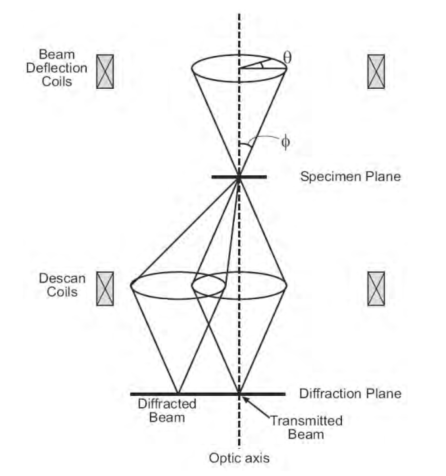
\includegraphics[width=0.7\linewidth]{fig/other/SPED-apparatus}
	\caption{Figure from \cite{sped-thesis}}
	\label{fig:precession}
\end{figure}

Scanning precession electron diffraction (SPED) is a modification of SED. \cref{fig:precession} shows the schematic of SPED. The electron beam is now tilted a fixed angle $\phi$ and precessed around the vertical axis. The beam will hit the sample at the same spot during the precession; only the direction of the incoming beam will be changed. The diffracted beam is also precessed so that the locations of the diffraction spots remain fixed during the precession. 

\begin{figure}
	\centering
	\begin{subfigure}{0.45\textwidth}
		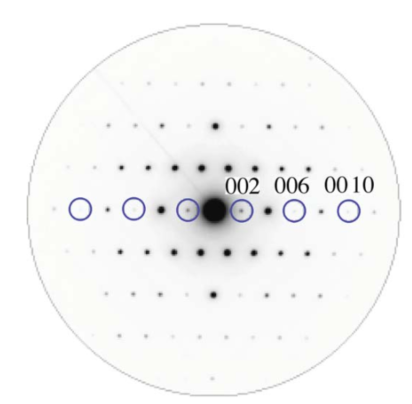
\includegraphics[width=\textwidth]{fig/other/dyndiff1}
		\caption{}
		\label{fig:dyndiff1}
	\end{subfigure}
	\hfill
	\begin{subfigure}{0.45\textwidth}
		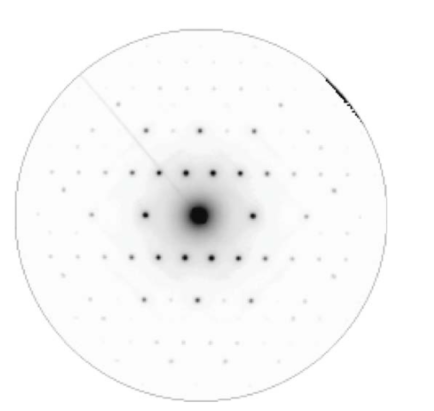
\includegraphics[width=\textwidth]{fig/other/dyndiff2}
		\caption{}
		\label{fig:dyndiff2}
	\end{subfigure}
	\caption{
		\label{fig:dyndiff}%
		From \cite{williams-carter}}
\end{figure}

There are several reasons why adding precession to electron diffraction gives better results. The perhaps most important is that the Ewald sphere is precessed in reciprocal space. This causes the Laue condition to be fulfilled for a higher number of reciprocal lattice points, resulting in more visible spots in the diffraction pattern. Another major improvement is the reduction of dynamical effects, in particular double diffraction, in the diffraction pattern. Double diffraction occurs when an electron is scattered twice, and can result in diffraction spots appearing even though they do not satisfy the Laue condition. As the beam is being precessed, dynamical effects are to a large extent averaged out \cite{williams-carter, sped-thesis}. \cref{fig:dyndiff} shows an example of how using a larger precession angle causes a reduction of dynamical effects.


\section{Data analysis}
	\subsection{(Introduction)}
	\subsection{Template matching}
	\label{sec:theory/template-matching}
Template matching is used for finding the location in a reference image where a template image fits best. The function \textit{MatchTemplate} in the python library OpenCV does this by sliding the template image over the reference image, and recording how well it fits at each point. This matching value is given as the normed square difference between the two images for each pixel in the reference image:
\begin{equation}
 R(x,y)= \frac{\sum_{x',y'} (T(x',y')-I(x+x',y+y'))^2}{\sqrt{\sum_{x',y'}T(x',y')^2 \cdot \sum_{x',y'} I(x+x',y+y')^2}}
 \label{eq:matching value}
\end{equation}

Here, $(x,y)$ are the coordinates of the reference image, $(x',y')$ the coordinates of the template, $I(x,y)$ is the value of the pixel $(x,y)$ in the reference image and $T$ likewise in the template. The matching value $R(x,y)$ can take any value between $0$ and $1$, where $0$ means a perfect match and $1$ a perfect mismatch.

	\subsection{Re-binning and rotating multidimensional data}
	\label{sec:rebin-rotate}
	
\begin{figure}
	\centering
	\begin{subfigure}{0.32\textwidth}
		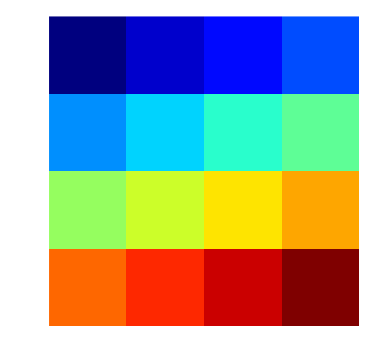
\includegraphics[width=\textwidth]{fig/other/rebin1}
		\caption{}
		\label{fig:rebin1}
	\end{subfigure}
	\hfill
		\begin{subfigure}{0.32\textwidth}
		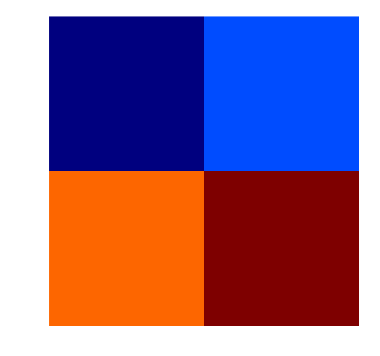
\includegraphics[width=\textwidth]{fig/other/rebin3}
		\caption{}
		\label{fig:rebin3}
	\end{subfigure}
	\hfill
		\begin{subfigure}{0.32\textwidth}
		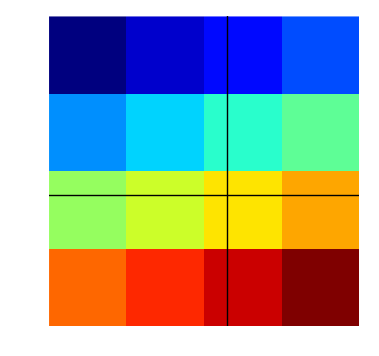
\includegraphics[width=\textwidth]{fig/other/rebin2}
		\caption{}
		\label{fig:rebin2}
	\end{subfigure}
\caption{
\label{fig:rebin}%
Rebin figures}
\end{figure}

Attempting to re-bin and rotate a multidimensional array can be problematic. A rotation that is not a multiple of 90 degrees will lead to jagged edges, and zero-values will have to be added to make it rectangular again. An even bigger problem occurs when re-binning an array. If the new lengths along each axis are divisors of the original lengths, it is relatively easy. \cref{fig:rebin1} shows a 4x4 array, where each value is visualized by a color. Rescaling this array by a factor of $s=2.0$ is simple as each value in the new array can be calculated as the mean of the corresponding 4 values (2x2 array) in the original array, resulting in the array in \cref{fig:rebin3}. This is called down-sampling, and causes information to be lost. Likewise, if re-binning the 4x4 by a factor of $s=0.5$, each value in the original array now corresponds to four values (2x2) in the new 8x8 array. These four values can simply be given the same value as the one in the original array. This procedure is called up-sampling, and new information is added.

However, if the new lengths of the array are not divisible by the original lengths, the re-binning procedure is no longer as easy to conceptualize. Imagine that instead of a two-dimensional array we now have a 3-dimensional one, where two of the dimensions are in real space and the third in signal space. This is the format of EDX data taken in STEM mode. Rescaling the real-space axes of this array will necessarily also change the signal axis. One way to solve this problem is to linearly interpolate the signal. Let the array in \cref{fig:rebin1} now denote the EDX dataset, with each color representing an EDX spectrum. If it is down-sampled by a scale factor of for example $s=2.3$, it will become a 2x2 array as before. However, as shown in \cref{fig:rebin2}, it is no longer as trivial. The top left value will now consist of the sum of the 2x2=4 top left values in the original matrix, plus 30 percent of the 3rd row and column. In the same way, the bottom right value will be the sum of the 2x2=4 bottom right values in the original matrix, plus 70 percent of the 3rd row and column. The result will be similar to \cref{fig:rebin3}, except that the colors (or spectra) will be slightly different. This process is called linear re-binning.

% !TEX encoding = UTF-8 Unicode
%!TEX root = thesis.tex
% !TEX spellcheck = en-US
%%=========================================
\chapter{Experimental}

\section{Equipment}

\section{Material}

\section{Dataset matching}
\label{sec:method/dataset matching}

Several methods were attempted in order to match the SPED and EDX datasets. The goal was that the matching would be performed automatically with no human input. For this to happen, the code would have to scale, rotate and translate one of the the datasets so that it fit the other. The EDX dataset taken at the intersection of the nanowire and the other elements deposited on it shows a relatively clear separation, and is also the dataset covering the biggest area of the sample. As the SPED dataset was taken over a larger area than the EDX dataset, it was decided to attempt to locate the position of the EDX dataset in the SPED dataset.

%The python library $\mathrm{imreg\_dft}$ \cite{imreg_dft} uses image registration to match two images. Several failed attempts were made using this technique. First, no processing was made to either dataset. The mean was taken in signal space in order to convert them into 2D images, and the intensities were scaled to the range $[0,255]$ so they would be uint8-images. The images were then input into the function, but the result did not come close. Several other attempts were done, following the same structure, except that the datasets were processed in different ways before being converted to 2D images:
%
%\begin{itemize}
%\item Principal component analysis (PCA) was performed on each dataset, and only the component most related to the GaAs nanowire was kept. The nanowire in each of the images now had a high intensity while all other areas were low in intensity.
%\item A similar result was obtained by inserting a virtual annulus in the SPED dataset, so that only a single diffraction spot corresponding to the nanowire was visible. In the EDX dataset, the EDX spectrum was cropped to only include the characteristic peaks corresponding to the nanowire.
%\item A virtual high-angle annular dark field aperture (virtual HAADF) was inserted in the SPED dataset, which was then compared to the DF image taken during the EDX session.
%\item .. background substraction? Thresholding
%\end{itemize}

%As none of these attempts gave any results, another and far more extensive python package, OpenCV \cite{open-cv}, was used instead. The ECC image alignment algorithm \cite{open-cv-ECC} can transform and fit an image using one of three different motions: Translation, euclidian or affine transformation. Here also, different preprocessing steps were taken to make the 2D images of the datasets more similar to each other. The affine transformation uses rotation, translation, scale and shear to fit the images. The euclidian transformation only rotates and translates, so one of the images was rotated before this algorithm was used. The rotation angle was estimated by measuring the angle between the same straight line (the intersection between the nanowire and the deposited elements) in both datasets, and the rotation was performed using the python library sci-kit image \cite{scikit-image}. Finally, the pure translation was attempted, and one of the images was rotated and scaled first. The scaling was performed by selecting the same two points in each datasets, and and using scikit-image to scale by the relative distance between them.
%
%Of these attempts, only the last attempt using the pure translation transformation gave results that were decent, but it was unstable and it was difficult to estimate the accuracy. It also required an unwanted amount of manual input from the user. It was then discovered that the metadata in HyperSpy contained accurate magnification numbers, so these were now used to scale the images relative to each other. It was then attempted to use another OpenCV algorithm, template matching \cite{open-cv-template-matching}, which was described in Section \ref{sec:++++++++}. This algorithm does not detect offset in rotation, so the SPED image was rotated using the manual technique described above.

% Actual solution

The python library OpenCV contains an algorithm which uses template matching, described in \cref{sec:theory/template-matching}, to find the best matching location of one image in another. The algorithm requires that the images are correctly scaled and rotated. To be used with this function, the two datasets first had to be processed to make them look more similar, and to enhance the border of the nanowire. The signal space of each of the datasets was limited to only include signals corresponding to the nanowire. For the SPED dataset, this was done by inserting a virtual annulus that covered only one diffraction spot, which was unique for the nanowire. Similarly, in the EDX dataset, the spectrum was cropped to only include the characteristic $K_\alpha$-peaks of Ga and As. The signal dimension of the datasets were then averaged out, in order to convert them into 2-dimensional arrays, or equivalently, gray-scale images.

The images were now rotated and rescaled. The rotation angle was estimated by selecting two points along the same straight line in both images and finding the angle between them. In the HyperSpy metadata of each of the datasets, a scaling factor giving the size of each pixel was given. The SPED image was rotated through the estimated angle, and the EDX image was rescaled by the ratio between the scaling factors. In order to limit the error caused by manual estimation of the rotational angle, the template matching algorithm was run 100 times for angles in the range $\pm3$\% of the manually estimated angle. In addition, because the contrast levels of the two images are not necessarily equal, the SPED image was multiplied by a gray-scale factor, ranging from 0.80 to 0.85 (this range was found experimentally to give the best results) through 30 steps. For each of the 30 $\times$ 100 iterations of the template matching algorithm, the matching value defined in \cref{eq:matching value} was calculated, and the angle and gray-scale factor giving the lowest matching value were obtained. ++WRITE ABOUT THIRD STEP

After finding the position of the EDX image in the SPED image, the full datasets were processed to enable them to share the same navigation window (define this?). First, the SPED dataset was rotated using T. Aarholt's \textit{rotate}-function \cite{aarholt-rotation}, which is currently awaiting implementation into HyperSpy. Then, the EDX dataset was rescaled and re-binned using K. MacArthur's function \textit{linear\_bin} \cite{kate-binning}, also awaiting implementation into HyperSpy. The functionality of this function is described in \cref{sec:rebin-rotate}. Lastly, a portion of the SPED dataset, corresponding to the location of the EDX image found earlier, was cut out. The two datasets now have the same number of pixels in real space, and each pixel corresponds to the same area of the sample. Using the \textit{Mirror navigation}-function in HyperSpyUI \cite{hyperspyUI}, the two datasets can be made to share a navigation window. 

It then remained to do this for the remaining datasets, all of were are smaller than the dataset used above. Instead of repeating the procedure, the HAADF image, which shows a large area of the sample, was used to find the positions of the remaining datasets with respect to the first. To do this, OpenCV template matching was used to locate the positions of all the datasets in the HAADF image. It was first attempted to use the EDX datasets, converted to images using the technique described earlier. This worked well for the datasets covering a relatively large region of the sample, but not for the smaller ones. Therefore, instead of the datasets, the survey images were used. These images are taken before the EDX recording, and shows a larger region of the sample (is this survey image also HAADF?). After image matching was complete, the matched region was cropped to the actual area of the EDX dataset. The coordinates of this area were found in the survey image's metadata in HyperSpy. 

Lastly, the positions of the remaining datasets had to be found in the SPED dataset. The datasets were again scaled and re-binned to fit the SPED dataset, but now also the coordinates in the HAADF image had to scaled to the SPED dataset, so that the correct area could be cropped out. This step has not been completed.

\section{Quantitative analysis}

\begin{figure}
	\centering
	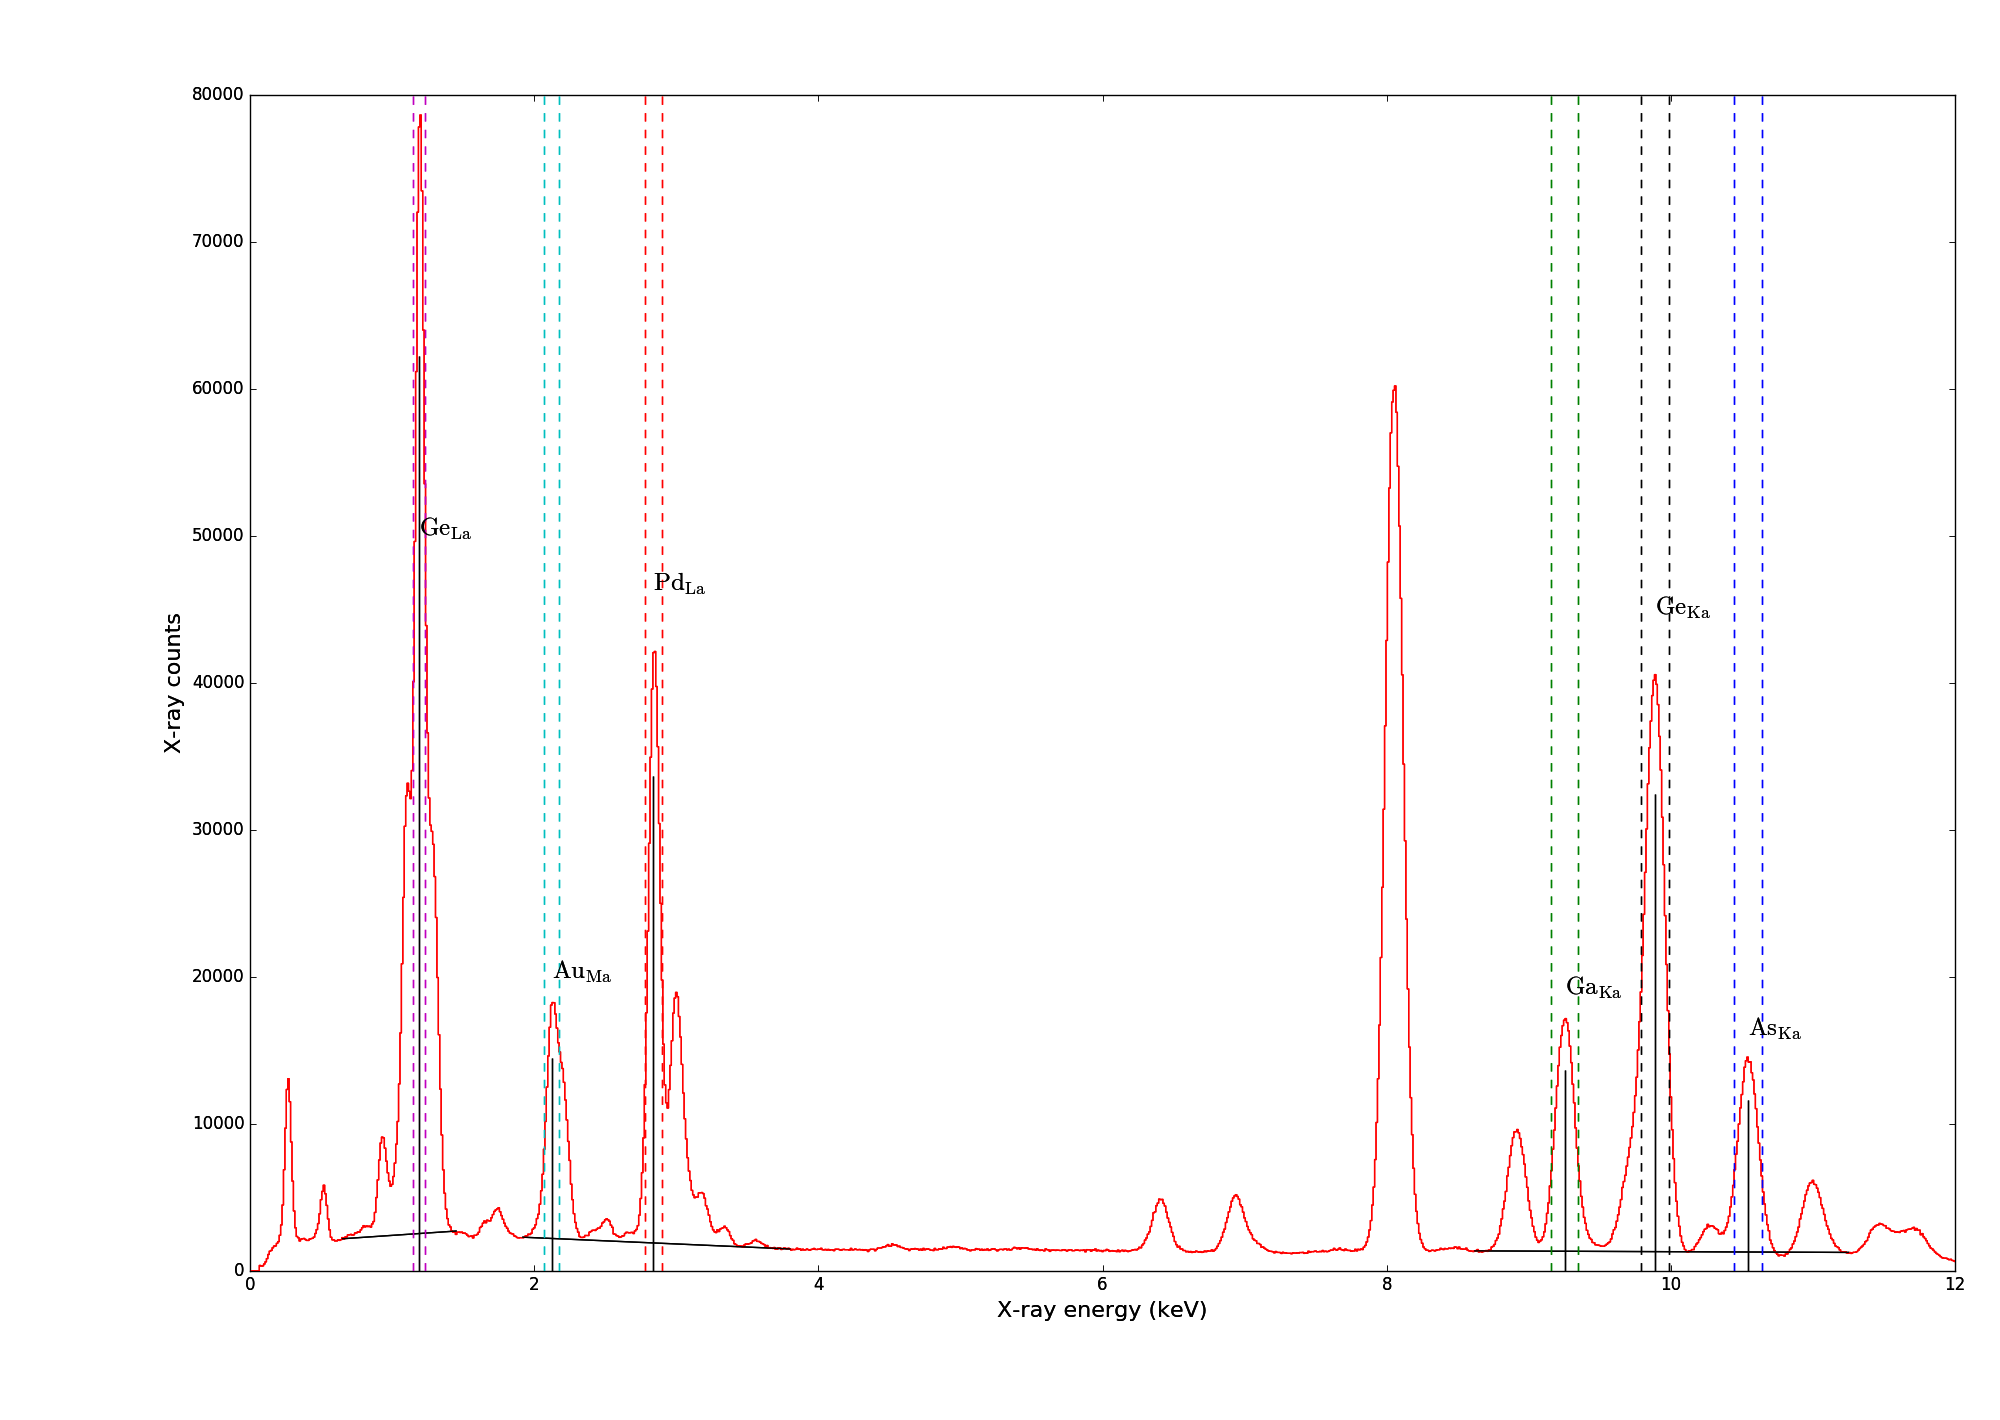
\includegraphics[width=0.7\linewidth]{fig/other/UnheatedA-full-spectrum2}
	\caption{}
	\label{fig:spectrum-with-info}
\end{figure}
The first step in the quantitative analysis was to determine the $\zeta$-factors of the elements in the sample. As this method had not yet been implemented into HyperSpy \cite{hyperspy}, the necessary code was acquired from the Master's thesis of A. Garmannslund \cite{andreas}. The thickness of the material was estimated using a thickness map (see Section ????). Background subtraction was performed by selecting an area of the background signal at both sides of each characteristic line, and drawing a line between the centers of these two areas. The intensities of the lines were then calculated by integrating over the peaks within an integration window of 1.2 FWHM. \cref{fig:spectrum-with-info} shows the characteristic X-ray peaks that have been used, the background that has been subtracted and the integration windows.

Thickness map

The quantification of the samples was performed using three different methods: The Cliff-Lorimer ratio technique, for which the necessary $k$-factors were obtained from the TEM software, the $\zeta$-factor method and the $\zeta$-factor method with background subtraction. HyperSpy was used for the first two of these methods, but absorption correction is at the time not been included in the software. The necessary code for this was also acquired from Garmannslund's thesis. All three techniques were used, in order to enable the results to be compared against each other. To verify the techniques, they were first used on the untreated sample whose composition is assumed to be known. They were then used on the heated sample in order to determine the composition at locations of interest.
% !TEX encoding = UTF-8 Unicode
%!TEX root = thesis.tex
% !TEX spellcheck = en-US
%%=========================================
\chapter{Results}

The results will be introduced in the same order as the experiments were conducted. First, the results of matching of one of the EDX datasets with the SPED dataset will be presented. This is followed the position matching of the various EDX datasets with the overview images. Lastly, the calculated $\zeta$-factors and the quantification of the samples using the $\zeta$-factor method and the Cliff-Lorimer technique are displayed.

\section{Dataset matching}

\cref{fig:edx-in-sped} shows the results of matching the largest EDX dataset with the SPED dataset. As explained in \cref{sec:method/dataset matching}, these images have been processed to be made more similar. \cref{fig:edx-in-sped} shows the processed EDX image and \cref{fig:edx-in-sped-rectangle} shows the processed SPED image with a rectangle indicating where the EDX image fit best. 

\begin{figure}
\begin{subfigure}{.5\textwidth}
	\centering
	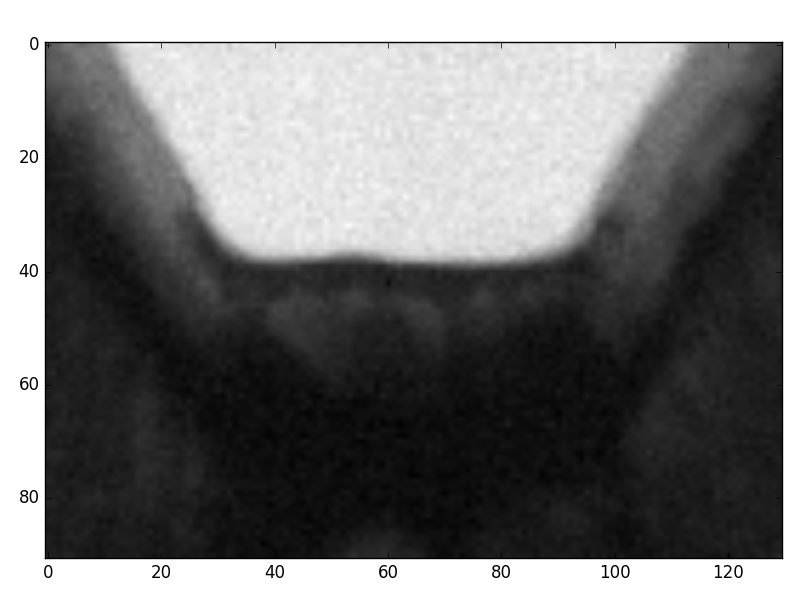
\includegraphics[width=\linewidth]{fig/se_image_in_sped_with_rectangle.png}
	\caption{++++++}
	\label{fig:edx-in-sped-edx}
\end{subfigure}%
\begin{subfigure}{.5\textwidth}
	\centering
	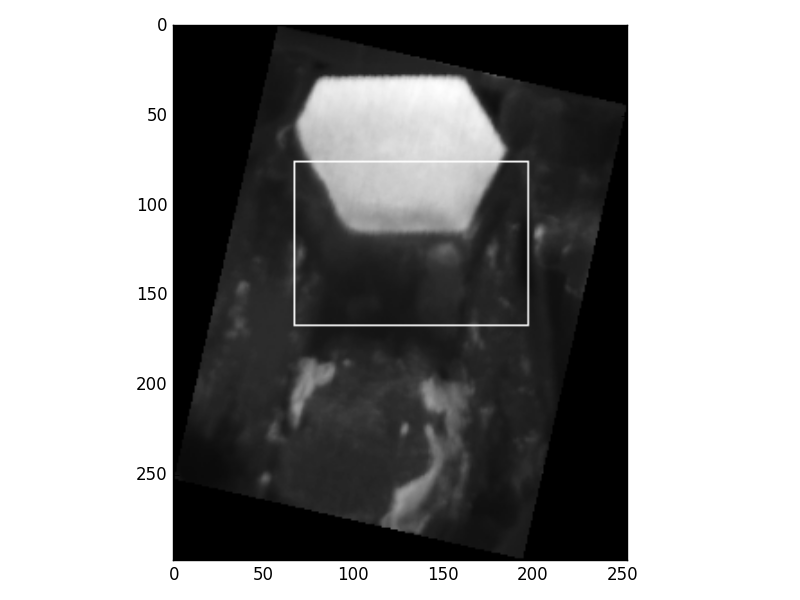
\includegraphics[width=\linewidth]{fig/sped-with-rectangle.png}
	\caption{++++++}
	\label{fig:edx-in-sped-rectangle}
\end{subfigure}
\caption{plots of....}
\label{fig:edx-in-sped}
\end{figure}

As the correct result is unknown, it is difficult to quantify the error in the fit. An attempt was made by looking at the difference between the matching value for the best position, shown in \cref{fig:edx-in-sped-rectangle}, and the higher values. The matching values are defined in \cref{eq:matching value}. \cref{fig:edx-sped-rectangle-match-graph} shows the relative error of the 100 best matching values with respect to the best match. 

\begin{figure}
	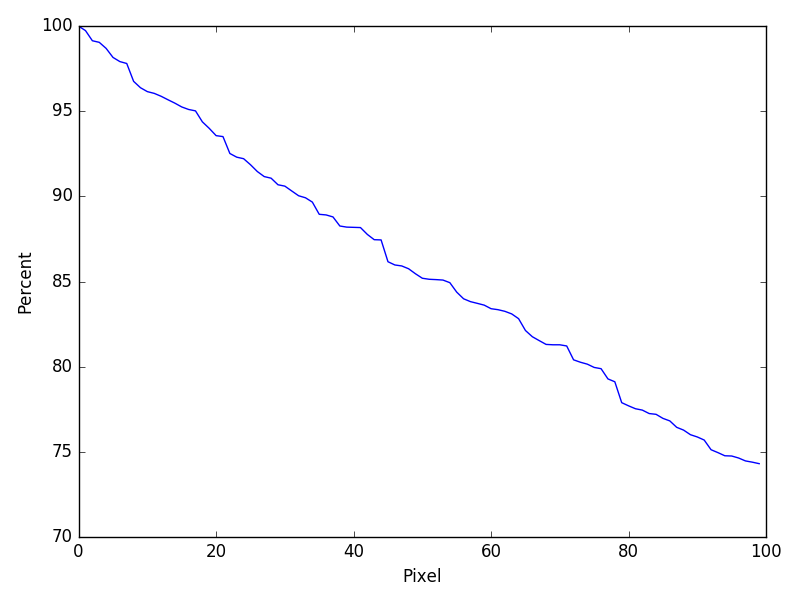
\includegraphics[width=0.7\linewidth]{fig/edx-sped-rectangle-match-graph.png}
	\caption{++++++}
	\label{fig:edx-sped-rectangle-match-graph}
\end{figure}

The results from locating the EDX datasets in the HAADF overview images are displayed in \cref{fig:nonheated-images-in-overview, fig:heated-images-in-overview} for the non-treated and the heat-treated samples, respectively. In the non-treated sample, the two datasets B and D were not correctly located in the overview image. The calculated location of dataset B was completely off, while the position of D was just slightly offset. The actual positions of these datasets were estimated by eye and marked in \cref{fig:nonheated-images-in-overview} as blue dotted rectangles. The rest of the datasets were located correctly, and their positions are shown as red rectangles. For the heat-treated sample, all the datasets that were included in the overview image were correctly located. However, the areas covered by two the datasets A and B were found to not be included in the overview image.

\begin{figure}
	\begin{subfigure}{.5\textwidth}
		\centering
		\includegraphics[width=\linewidth]{"fig/nonheated-images-in-overview (correct)3"}
		\caption{}
		\label{fig:nonheated-images-in-overview}
	\end{subfigure}%
	\begin{subfigure}{.5\textwidth}
		\centering
		\includegraphics[width=\linewidth]{"fig/nonheated-matching-values"}
		\caption{}
		\label{fig:nonheated-matching-values}
	\end{subfigure}
\end{figure}

\begin{figure}
	\begin{subfigure}{.5\textwidth}
		\centering
		\includegraphics[width=\linewidth]{"fig/heated-images-in-overview-ink2"}
		\caption{}
		\label{fig:nonheated-images-in-overview}
	\end{subfigure}%
	\begin{subfigure}{.5\textwidth}
		\centering
		\includegraphics[width=\linewidth]{"fig/heated-matching-values"}
		\caption{}
		\label{fig:nonheated-matching-values}
	\end{subfigure}
\end{figure}

The accuracy of the matching for the different datasets are shown in \cref{fig:nonheated-matching-values} for the non-heated sample, and in \cref{fig:heated-matching-values} for the heated values. The horizontal axis shows the different datasets while the vertical axis is the matching value in percent, where $\SI{100}{\percent}$ is defined to be the matching value of the dataset covering the biggest area in each respective sample. The matching of this dataset is assumed to be the most trustworthy due to there being fewer potential locations that resemble the actual location, as there are several distinct features. For the smaller datasets, or more accurately, the datasets with smaller survey images, there might be several different locations in the overview image that all give a fairly good match.


In both figures, the red star is the value of the dataset used as reference, the red circles are the correctly matched datasets while the blue squares are the datasets that resulted in a wrong location. The non-heated sample (\cref{fig:nonheated-matching-values}) shows high values for all the correctly located datasets, and significantly lower values for the wrongly located ones. In addition, it must be noted that the exact location of dataset F was impossible to verify visually due to the survey image not being large enough to distinguish specific features. In the heated sample (\cref{fig:heated-matching-values}), all the red correctly located datasets have high values while the datasets that were not present in the reference image have distinguishably lower values.

\section{Determination of $\zeta$-values}

The calculated $\zeta$-values for all the elements present in the sample are presented in \cref{tab:non-heated zeta-values}, along with which dataset was used to calculate them. All datasets are from the unheated sample except for C*, which is from the heated one.

\begin{table}
	\caption{...}
	\begin{center}
	\begin{tabular}{ccc}

	Element & Dataset & $\zeta$\\ 
	\midrule
	\hline
	Ga & C* & 582\\
	Ga & A  & 608\\
	As & C* & 689\\
	As & A  & 706\\
	Ge & B  & 732\\
	Ge & D  & 741\\
	Ge & A  & 748\\
	Pd & E  & 1248\\
	Pd & A  & 1284\\
	Pd & B  & 1318\\
%	Au & B  & 3450\\ 
%	Au & C  & 3473\\
	Au & B & 2397\\
	Au & C & 2387\\
	\hline
	\end{tabular} 
	\end{center}
	\label{tab:non-heated zeta-values}
\end{table}

These values have been 


\section{Quantification}

The compositions of the unheated and the heated samples have been quantified using the Cliff-Lorimer ratio method and the $\zeta$-factor method with and without absorption correction. The composition of the unheated sample is known, and can therefore used as a reference for the accuracy of the quantization of the heated sample, whose composition is largely unknown.

\begin{figure}
	\begin{subfigure}{.5\textwidth}
		\centering
		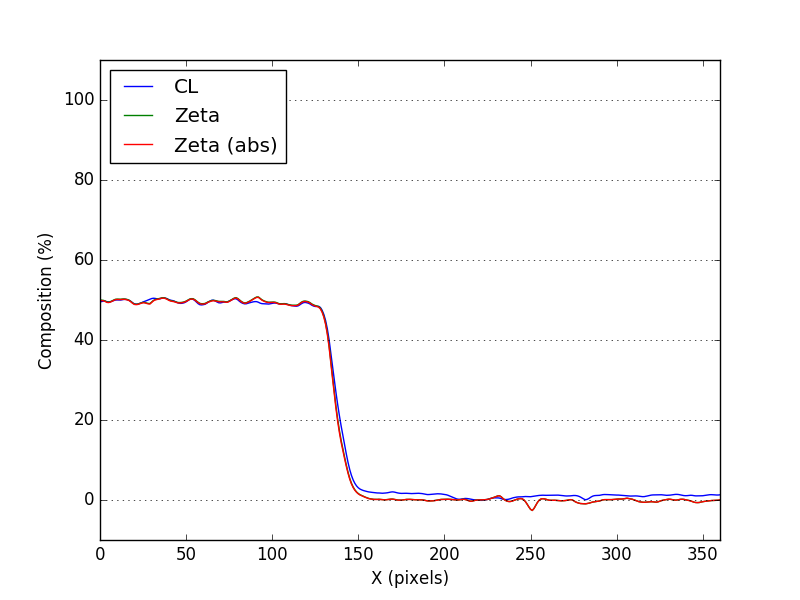
\includegraphics[width=\linewidth]{fig/q/1_ga2}
		\caption{++++++}
		\label{fig:zeta_area1_ga}
	\end{subfigure}%
	\begin{subfigure}{.5\textwidth}
		\centering
		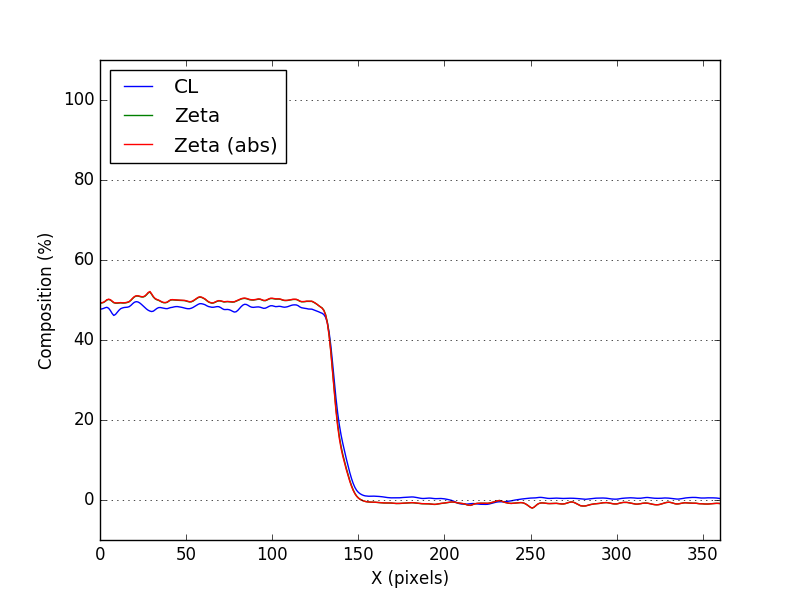
\includegraphics[width=\linewidth]{fig/q/1_as2}
		\caption{++++++}
		\label{fig:zeta_area1_as}
	\end{subfigure}
		\begin{subfigure}{.5\textwidth}
			\centering
			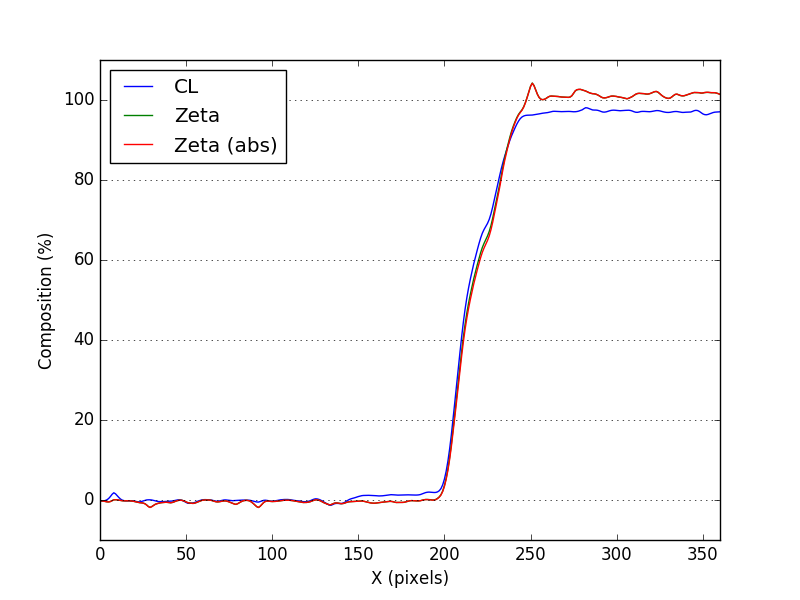
\includegraphics[width=\linewidth]{fig/q/1_ge2}
			\caption{++++++}
			\label{fig:zeta_area1_ge}
		\end{subfigure}%
		\begin{subfigure}{.5\textwidth}
			\centering
			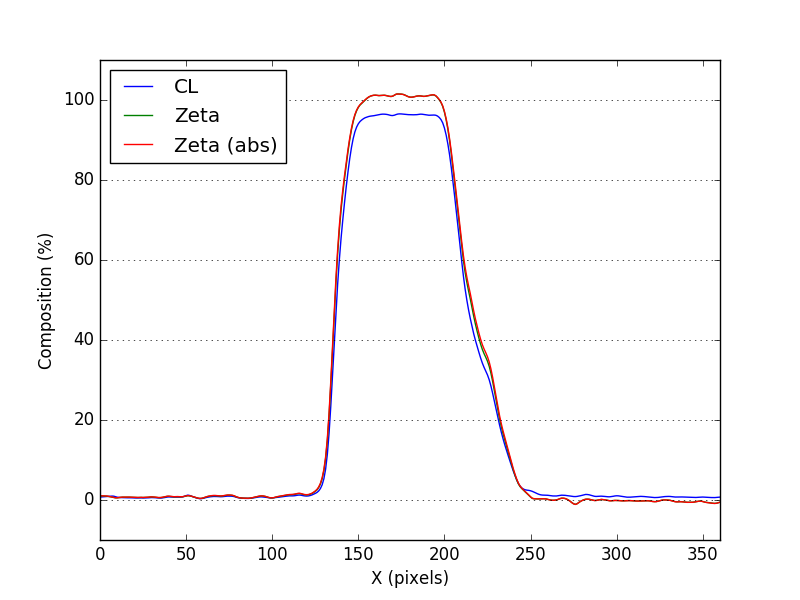
\includegraphics[width=\linewidth]{fig/q/1_pd2}
			\caption{++++++}
			\label{fig:zeta_area1_pd}
	\end{subfigure}
		\begin{subfigure}{.5\textwidth}
			\centering
			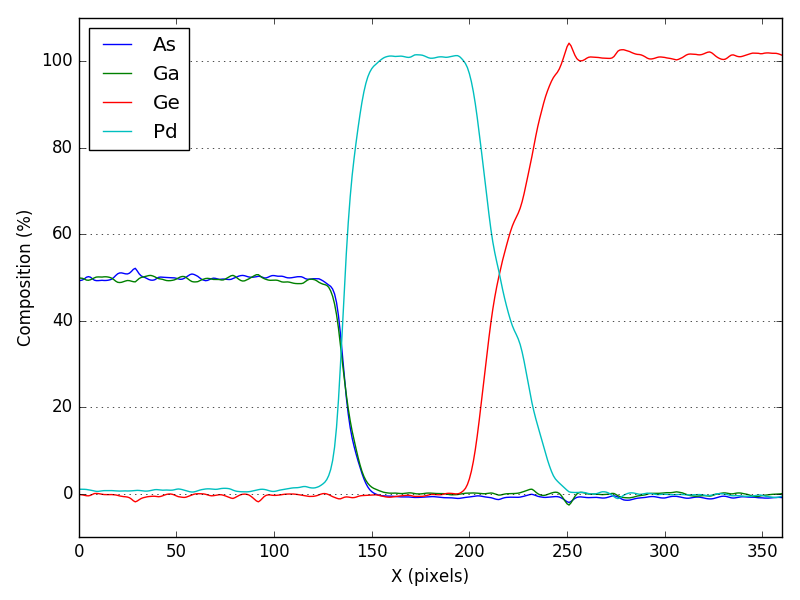
\includegraphics[width=\linewidth]{fig/q/1_all_abscorr2}
			\caption{++++++}
			\label{fig:zeta_area1_all}
	\end{subfigure}%
	\begin{subfigure}{.5\textwidth}
		\centering
		\newlength\imageheight
%		\settoheight\imageheight{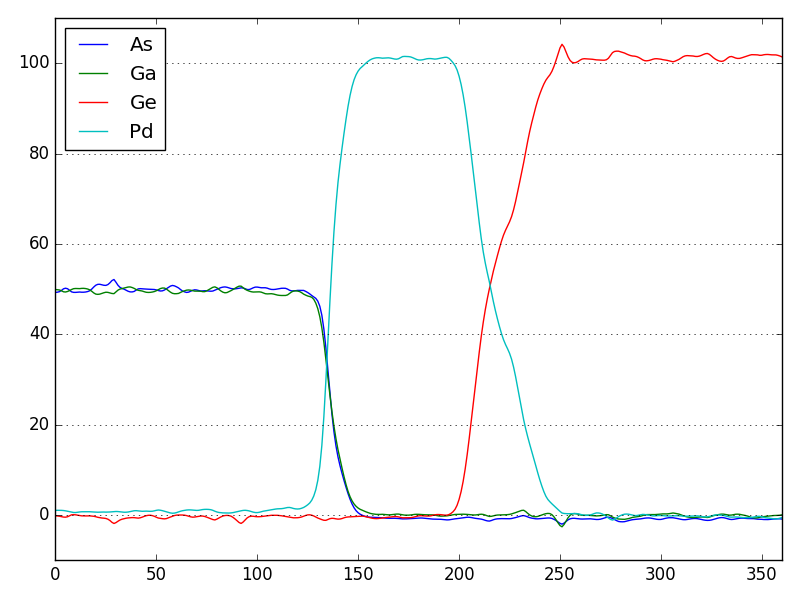
\includegraphics{fig/q/1_all_abscorr}}
%		\newlength\imagewidth
%		\settowidth\imagewidth{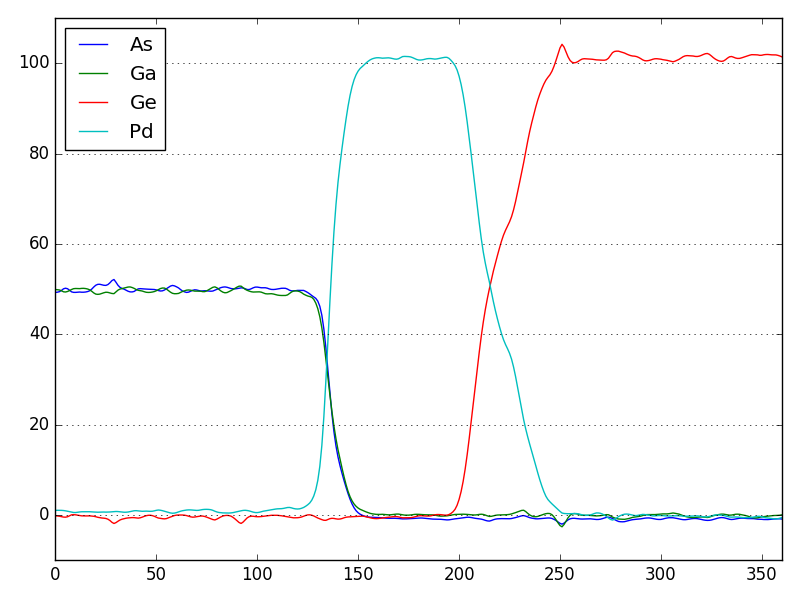
\includegraphics{fig/q/1_all_abscorr}}
		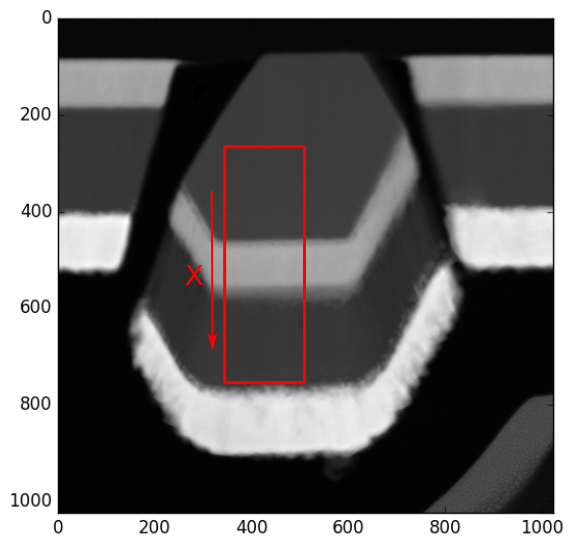
\includegraphics[width=.68\linewidth]{fig/q/1_overview3}
		\caption{++++++}
		\label{fig:zeta_area1_overview}
	\end{subfigure}
	\caption{plots of....}
	\label{fig:zeta_area1}
\end{figure}

\begin{figure}
	\begin{subfigure}{.5\textwidth}
		\centering
		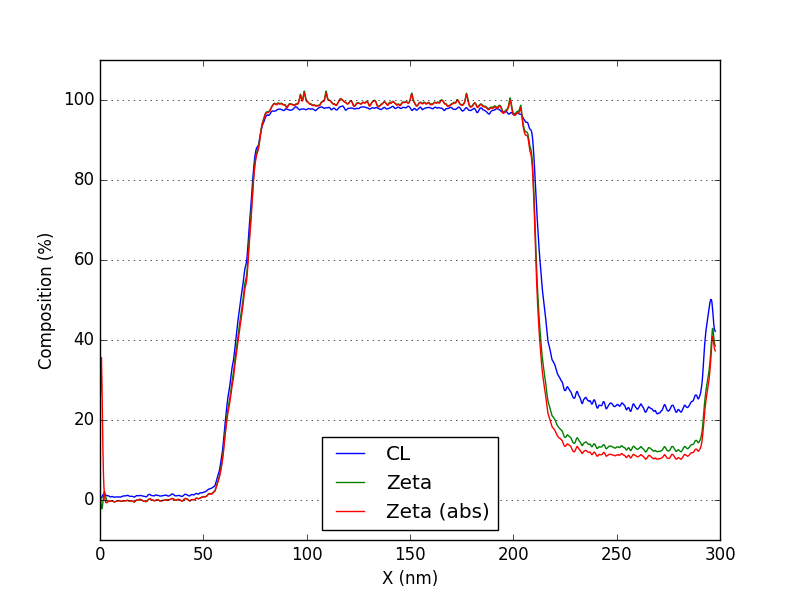
\includegraphics[width=\linewidth]{fig/q/2_ge}
		\caption{++++++}
		\label{fig:zeta_area1_ga}
	\end{subfigure}%
	\begin{subfigure}{.5\textwidth}
		\centering
		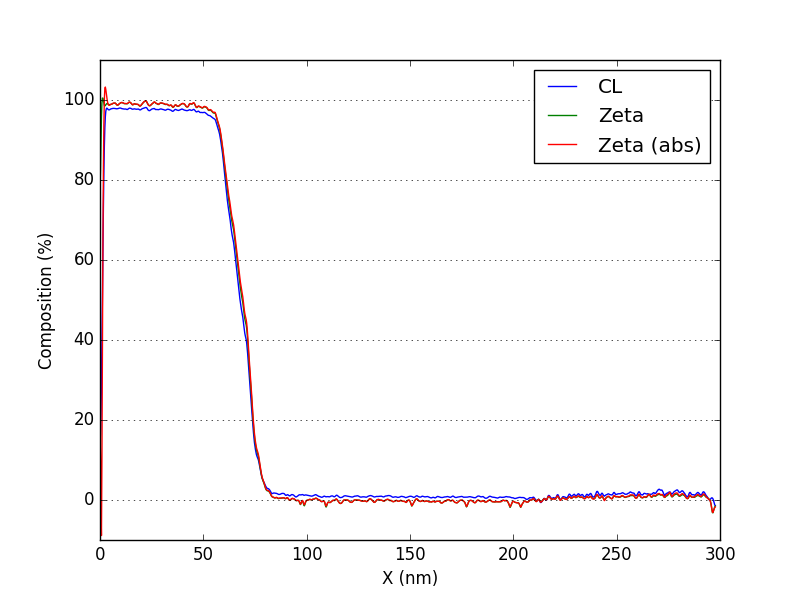
\includegraphics[width=\linewidth]{fig/q/2_pd}
		\caption{++++++}
		\label{fig:zeta_area1_as}
	\end{subfigure}
	\begin{subfigure}{.5\textwidth}
		\centering
		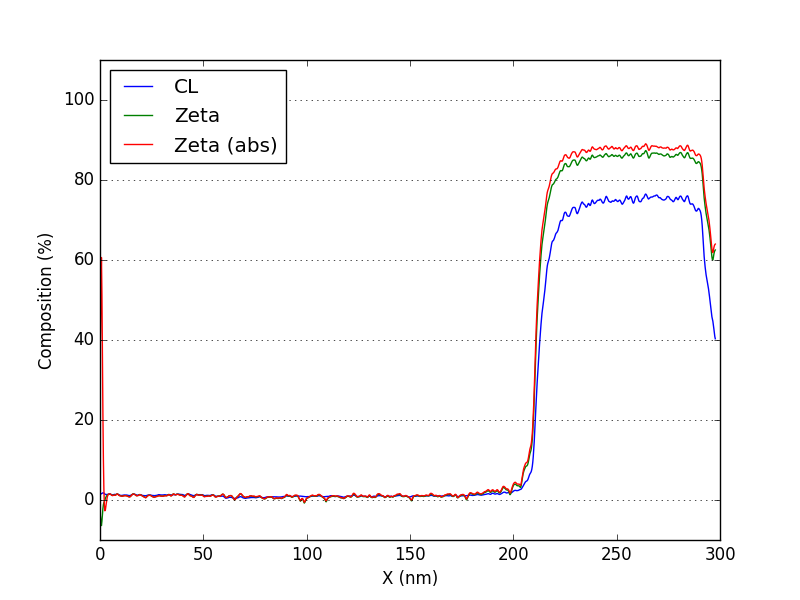
\includegraphics[width=\linewidth]{fig/q/2_au}
		\caption{++++++}
		\label{fig:zeta_area1_ge}
	\end{subfigure}%
	\begin{subfigure}{.5\textwidth}
		\centering
		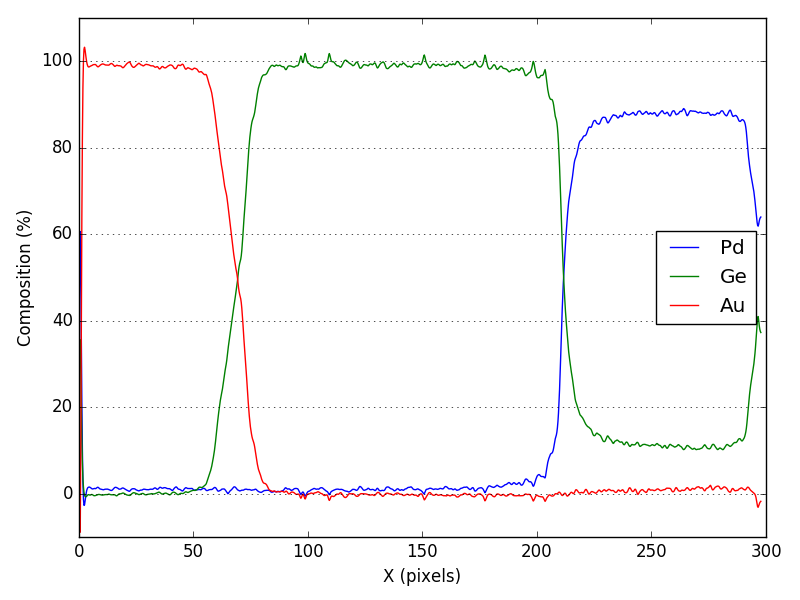
\includegraphics[width=\linewidth]{fig/q/2_all_abscorr}
		\caption{++++++}
		\label{fig:zeta_area1_all}
	\end{subfigure}
		\centering
	\begin{subfigure}{.5\textwidth}
%		\newlength\imageheight
		%		\settoheight\imageheight{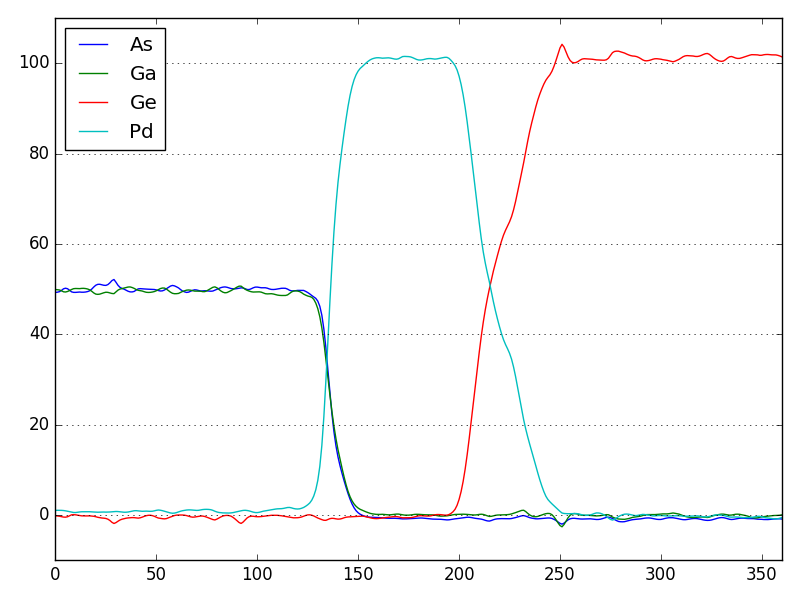
\includegraphics{fig/q/1_all_abscorr}}
		%		\newlength\imagewidth
		%		\settowidth\imagewidth{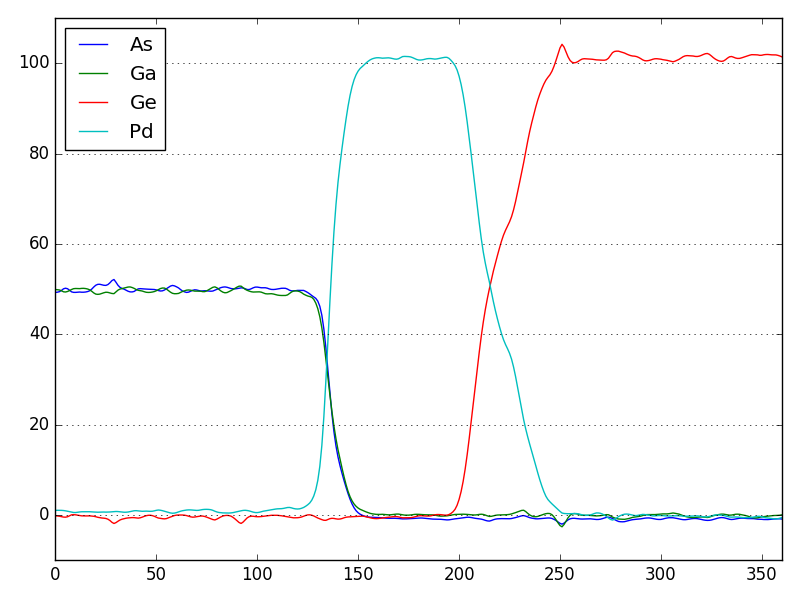
\includegraphics{fig/q/1_all_abscorr}}
		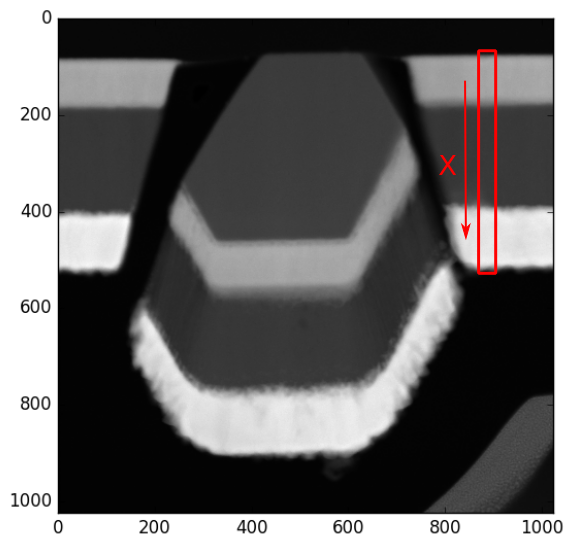
\includegraphics[width=.68\linewidth]{fig/q/2_overview}
		\caption{++++++}
		\label{fig:zeta_area2_overview}
	\end{subfigure}
	\caption{plots of....}
	\label{fig:zeta_area2}
\end{figure}
% Include more chapters as required.
%%=========================================
\appendix
% !TEX encoding = UTF-8 Unicode
%!TEX root = thesis.tex
% !TEX spellcheck = en-US
%%=========================================

\chapter{Acronyms}
\begin{description}
\item[FTA] Fault tree analysis
\item[MTTF] Mean time to failure
\item[RAMS] Reliability, availability, maintainability, and safety
\end{description}
% !TEX encoding = UTF-8 Unicode
%!TEX root = thesis.tex
% !TEX spellcheck = en-US
%%=========================================

\chapter{Additional Information}
This is an example of an Appendix. You can write an Appendix in the same way as a chapter, with sections, subsections, and so on.

%%=========================================
\section{Introduction}

%%=========================================
\subsection{More Details}
% Include more appendices as required.
%%=========================================
\bibliographystyle{plain}
%\addcontentsline{toc}{chapter}{\bibitem}
\bibliography{refs}
%%=============================================

\end{document}
